\begin{figure}[h]
  \begin{minipage}{\textwidth}
    \centering
    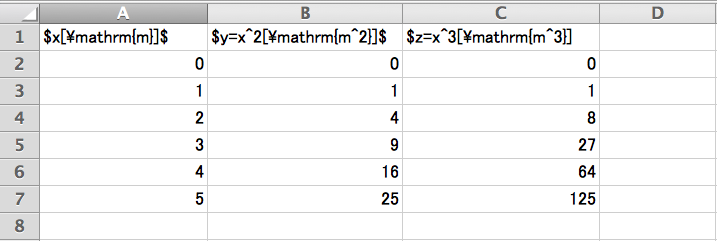
\includegraphics[height=.2\textwidth]{./contents/3_latex_knowhow/figure/table_writing_1.png}
    \subcaption{Write a table you want to write on Excel}\figlab{table_writing_1.png}
    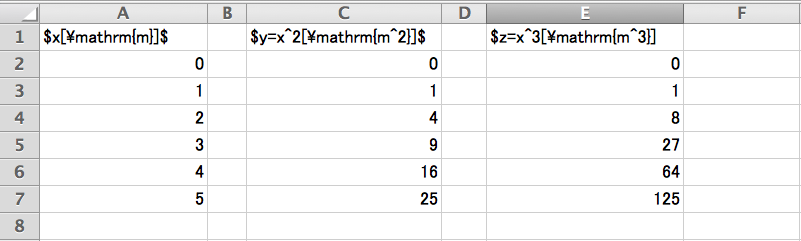
\includegraphics[height=.2\textwidth]{./contents/3_latex_knowhow/figure/table_writing_2.png}
    \subcaption{Add blank columns within each column}\figlab{table_writing_2.png}
    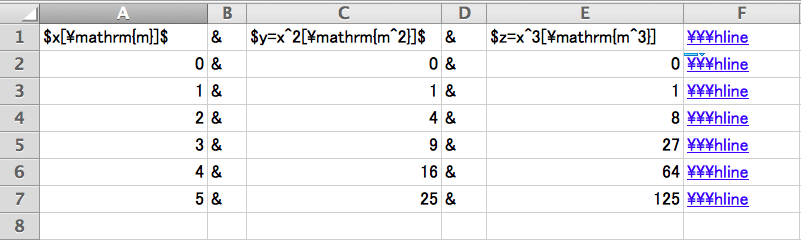
\includegraphics[height=.2\textwidth]{./contents/3_latex_knowhow/figure/table_writing_3.png}
    \subcaption{Fill \& \!s in the blanks column and \textbackslash\textbackslash\textbackslash hline in the last column}\figlab{table_writing_3.png}
    \begin{minipage}{.6\textwidth}
      \begin{screen}
        \centering
        \small{
        \begin{verbatim} 
\begin{table}[htbp]
\centering
\caption{Title}
\tablab{Title}
\begin{tabular}{ l | c | r } \hline\hline
   **here**
\end{tabular}
\end{table}\end{verbatim}}
      \end{screen}
    \end{minipage}
    \subcaption{Copy and paste the table area into **here**}\figlab{table_writing_4}
  \end{minipage}
  \caption{Example of writing \tabref{Title}}\figlab{Example of writing a table}
\end{figure}